%auto-ignore
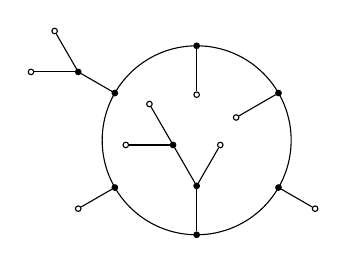
\begin{tikzpicture}

\def\rad{1.2cm}
\def\angdist{60}
\def\posa{90}
\def\extlen{0.6cm}

\tikzset{point/.style = {draw, circle, fill=black, minimum size=2pt,inner sep=0pt}}


\coordinate (C1) at (0,0) {};

\path (C1) node[point] (C11)  at +(\posa:\rad) {};
\path (C1) node[point] (C12)  at +(\posa+\angdist:\rad) {};
\path (C1) node[point] (C13)  at +(\posa+2*\angdist:\rad) {};
\path (C1) node[point] (C14)  at +(\posa+3*\angdist:\rad) {};
\path (C1) node[point] (C15)  at +(\posa+4*\angdist:\rad) {};
\path (C1) node[point] (C16)  at +(\posa+5*\angdist:\rad) {};


\draw (C1) circle (\rad);

% C1
\path (C1) to coordinate[pos=1-\extlen/\rad,point,style={fill=white}] (C111) (C11);
\draw (C11) -- (C111);


% C2
\path (C1) to coordinate[pos=1+\extlen/\rad,point] (C121) (C12);
\path (C121) node[point,style={fill=white}] (C1211)  at +(\posa+\angdist+30:\extlen) {};
\path (C121) node[point,style={fill=white}] (C1212)  at +(\posa+\angdist-30:\extlen) {};

\draw (C12) -- (C121);
\draw (C121) -- (C1211);
\draw (C121) -- (C1212);

% C3
\path (C1) to coordinate[pos=1+\extlen/\rad,point,style={fill=white}] (C131) (C13);
\draw (C13) -- (C131);


% C4
\path (C1) to coordinate[pos=1-\extlen/\rad,point] (C141) (C14);
\path (C141) node[point] (C142)  at +(120:\extlen) {};
\path (C141) node[point,style={fill=white}] (C143)  at +(60:\extlen) {};
\path (C142) node[point,style={fill=white}] (C1421)  at +(180:\extlen) {};
\path (C142) node[point,style={fill=white}] (C1422)  at +(120:\extlen) {};
\draw (C14) -- (C141);
\draw (C141) -- (C142);
\draw (C141) -- (C143);
\draw (C142) -- (C1421);
\draw (C142) -- (C1422);

% C5
\path (C1) to coordinate[pos=1+\extlen/\rad,point,style={fill=white}] (C151) (C15);
\draw (C15) -- (C151);

% C6
\path (C1) to coordinate[pos=1-\extlen/\rad,point,style={fill=white}] (C161) (C16);
\draw (C16) -- (C161);

\end{tikzpicture}